\section{Structure}
In this section we will be describing the overall structure of the program, through class diagrams.

\fxnote{Remove some of this shit..}

\subsection{Individual class description}
The \textbf{Foodplan} class describes a schedule of planned meals that a user can administrate and follow.
It can consists of 0 to many meals.

The \textbf{Meal} class contains information about a meal and when to make/eat it. It consists of recipes.

\textbf{Recipes} consists of \textbf{Food}.

\subsection{Class diagram description}
The class diagram is structured with \textbf{Food} as the central class. Food objects can be part of a \textbf{Shopping List}, a user \textbf{Inventory}, or be part of a \textbf{Recipe}.A \textbf{Recipe} is part of a \textbf{Meal} that in turn is part of a combined \textbf{Foodplan}.

\begin{figure}[H]
	\centering
	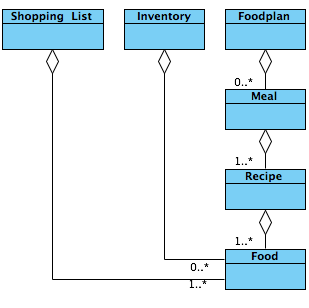
\includegraphics[width=0.50\textwidth]{Grafik/FoodPlanner/FoodPlannerClassDiagram.png}
	\caption{Relation between classes.}
\end{figure}

\fxnote{Update diagram}